\chapter{Modellbildung}

Ein Ziel dieser Arbeit besteht darin, für die am PtU der TU Darmstadt entwickelte und konstruierte 3D-Servo-Presse ein Black-Box-Modell zu entwickeln. Für die Bestimmung der Eingangs- und Ausgangsgrößen für das Modell ist die Erläuterung des Aufbaus und der Funktionsweise der 3D-Servo-Presse notwendig. Daraufhin folgen die Festlegung der System- und Modellgrenzen, die Vorgehensweise bei der experimentellen Datenermittlung und einige Erläuterungen zur der eingesetzten Software für die Modellbildung. Im Anschluss erfolgt die Modellbildung der 3D-Servo-Presse mittels verschiedener neuronaler Netze. Die entwickelten Modelle werden dann in Bezug auf ihre Approximationsfähigkeit, Trainingszeit, Robustheit, ihr Interpolations- und Extrapolationsverhaltens untersucht.

\section{Aufbau der 3D-Servo-Presse}

Wie in Abbildung \ref{fig:3d-servo} zu erkennen ist, befindet sich das Pressengetriebe im oberen und der Arbeitsbereich mit dem Stößel im unteren Bereich.

\begin{figure} [h]
	\centering
	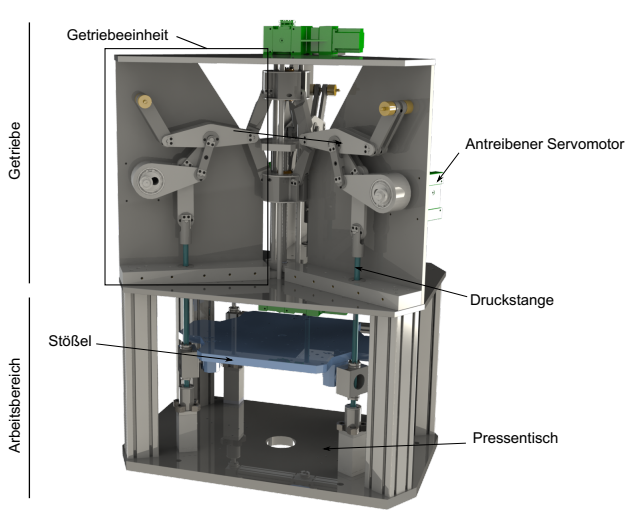
\includegraphics[width=0.75\textwidth]{images/3D-Servo-Presse}
	\caption{Oberer Pressenaufbau der 3D-Servo-Presse mit geöffnetem Getriebekasten \cite{Rakowitsch.2018}}
	\label{fig:3d-servo}
\end{figure}

Das Pressengetriebe besteht aus insgesamt drei Getriebeeinheiten, welche um $120^\circ$ versetzt sind. Der Antrieb jeder Getriebeeinheit erfolgt über einen Servo-Motor, dessen Rotationsbewegung über ein Koppeltriebe in eine translatorische Hubbewegung der zum Getriebe gehörende Druckstange umgesetzt wird, siehe Abbildung \ref{fig:koppel}.

\begin{figure} [h]
	\centering
	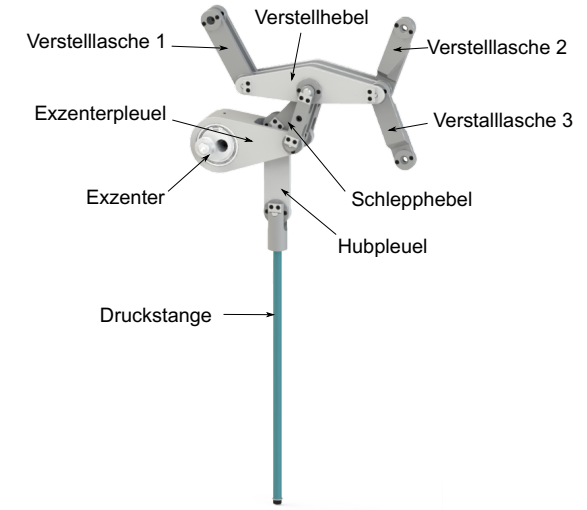
\includegraphics[width=0.65\textwidth]{images/exzenter}
	\caption{Koppelgetriebe mit Getriebeelementen zur Transformation der rotatorischen Bewegung des Servo-Motors in eine Hubbewegung der Druckstange \cite{Rakowitsch.2018}}
	\label{fig:koppel}
\end{figure}


Gelenke verbinden dabei die drei Druckstangen mit dem Stößel. Für eine rein translatorische Hubbewegung des Stößels verfahren alle drei Druckstangen gleichermaßen. Verfahren die drei Druckstangen unterschiedlich, kommt es zu einer Schrägstellung des Stößels. Jede der drei Getriebeeinheiten ist wiederum mit einer sich im Zentrum befindenden Verstelleinheit verbunden, siehe Abbildung, \ref{fig:verstelleinheit}.

Die Verstelleinheit besteht aus Führungsstangen und zwei übereinander angeordneten Spindeln, wobei jede Spindel durch einen Servo-Motor verstellt werden kann. Durch die Verstellung der oberen und der unteren Spindel findet die Einstellung des oberen und des unteren Totpunktes für die Druckstange statt. Die Einstellung des oberen und des unteren Totpunktes gilt dabei für jede Getriebeeinheit, da jede Getriebeeinheit mit der gleichen Verstelleinheit verbunden ist. Die Höhenverstellung jeder der drei Druckstangen ist also bedingt durch die Verstellung der oberen und unteren Spindel, genannt $s_o$ und $s_u$, und durch den Exzenterwinkel $\varphi_{exz}$, siehe Abbildung \ref{fig:prinzipskizze}.




Das Pressenmodell wird für eine rein translatorische Hubbewegung des Stößels entwickelt. Damit ist die Höhenverstellung aller drei Druckstangen identisch. Die Höhenverstellung der drei Druckstangen entspricht somit auch der Höhenverstellung des Stößels. 
Damit ist es zweckmäßig, ein Pressenmodell zu entwickeln, welches die Eingangsgrößen (obere Verstellung der Spindel $s_o$, untere Verstellung der Spindel $s_u$ und der Exzenterwinkel $\varphi_{exz}$) in die Höhenverstellung $y$ des Stößels als Ausgangsgröße transformiert. 

\begin{figure} [H]
	\centering
	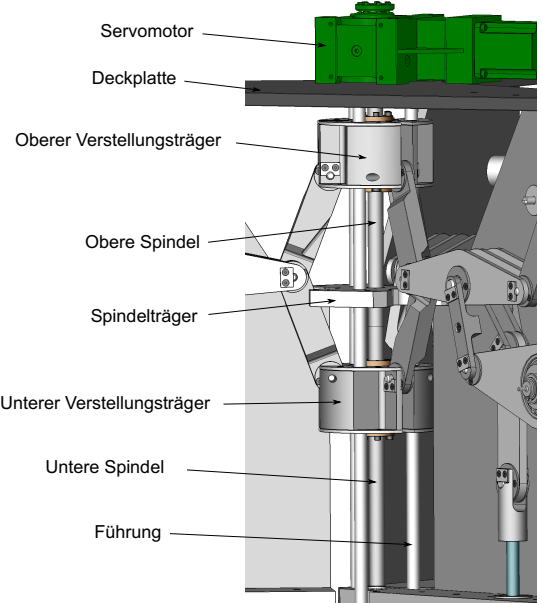
\includegraphics[width=0.6\textwidth]{images/verstelleinheit}
	\caption{Verstelleinheit zur Einstellung des oberen und unteren Totpunktes für die Druckstangen \cite{Rakowitsch.2018}}
	\label{fig:verstelleinheit}
\end{figure}

\begin{figure} [H]
	\centering
	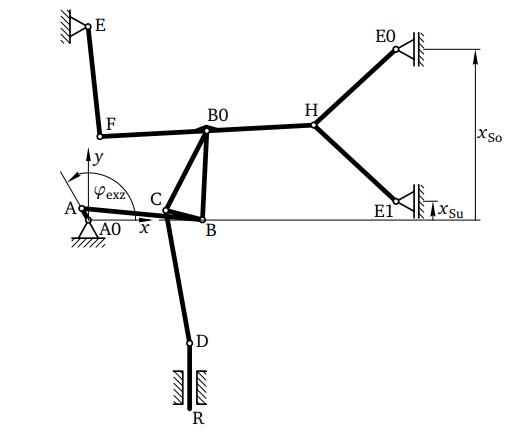
\includegraphics[width=0.65\textwidth]{images/prinzipskizze}
	\caption{Prinzipskizze des Getriebes \cite{Rakowitsch.2018}}
	\label{fig:prinzipskizze}
\end{figure}


\section{Definition der System- und Modellgrenzen}


Wie in letzten Abschnitt erklärt, ergibt sich die Höhenverstellung des Stößels $y$ aus der oberen Spindelverstellung $s_o$, der unteren Spindelverstellung $s_u$ und dem Exzenterwinkel $\varphi_{exz}$. Bei der Ermittlung der Messdaten findet eine rein translatorische Hubbewegung des Stößels statt, sodass die Neigung des Stößels um eine horizontale Ebene als potentielle weitere Ausgangsgröße wegfällt. Das Black-Box-Modell, welche die Eingangsgrößen in die Ausgangsgrößen transformiert, ist in dieser Arbeit ein  neuronales Netz, siehe Abbildung \ref{fig:blackbox}.

\begin{figure} [H]
	\centering
	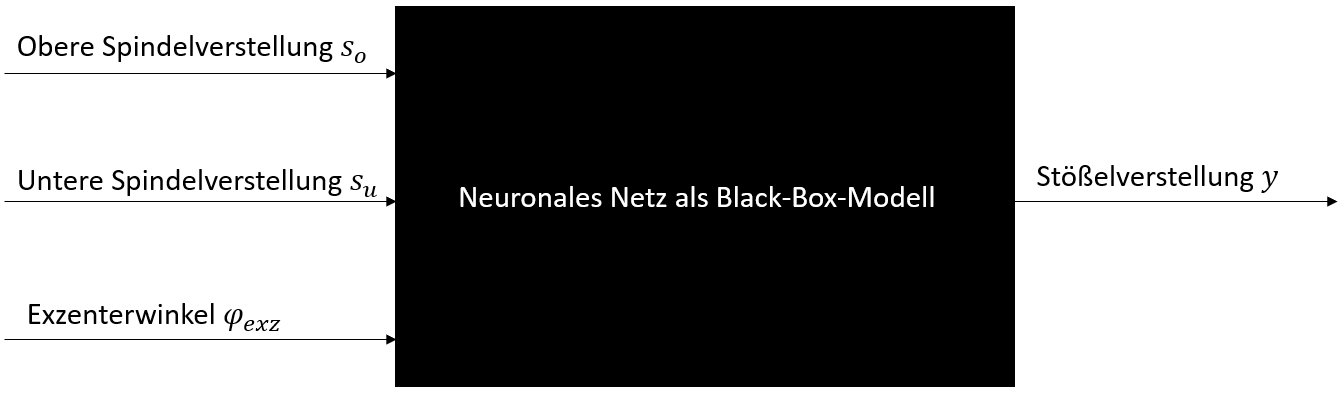
\includegraphics[width=0.85\textwidth]{images/blackbox}
	\caption{Neuronales Netz als Modellstruktur}
	\label{fig:blackbox}
\end{figure}


\section{Verwendete Software}
Für die Entwicklung neuronaler Netze zur Modellbildung der 3D-Servo-Presse kommt die Neural Network Toolbox\texttrademark  der MathWorks Inc. zum Einsatz. Für eine ausführliche Dokumentation der Neural Network Toolbox\texttrademark  sei auf \cite{Beale.2018} verwiesen. Die Neural Network Toolbox\texttrademark bietet die Möglichkeit, MLP-, RBF, GRNN-Netze und dynamische Netze, wozu das \textit{Nonlinear Autoregressive with External Input (NARX)}-, das \textit{Nonlinear Autoregressive (NAR)}- und das \textit{Nonlinear Input-Output}-Netz gehören, zu entwickeln. Wie in Abschnitt \ref{cha_ff} erklärt, kommen bei neuronalen Netzen Algorithmen zur Minimierung der Fehlerfunktion bei der Adaption der Netzwerkgewichte zum Einsatz. Die Neural Network Toolbox\texttrademark bietet insgesamt folgende zwölf Algorithmen an:

\begin{itemize}
	\item Levenberg-Marquardt (trainlm)
	\item Bayesian Regularization  (trainbr) 
	\item BFGS Quasi-Newton (trainbfg)
	\item Resilient Backpropagation (trainrp)
	\item Scaled Conjugate Gradient (trainscg)
	\item Conjugate Gradient with Powell/Beale Restarts (traincgb)
	\item Fletcher-Powell Conjugate Gradient (traincgf)
	\item Polak-Ribiére Conjugate Gradient (traincgp)
	\item One Step Secant (trainoss)
	\item Variable Learning Rate Gradient Descent (traingdx)
	\item Gradient Descent with Momentum (traingdm)
	\item Gradient Descent (traingd)
\end{itemize} 


\section{Trainingsdaten}

Das Training des neuronalen Netzes findet mit Hilfe von Trainingsdaten statt. Im Rahmen dieser Arbeit liegt zum einen ein Simulationsmodell der 3D-Servo-Presse vor, welches Trainingsdaten erzeugt. Zum anderen liegen experimentell ermittelte Trainingsdaten vor. Die mit Hilfe des Simulationsmodells erzeugten Trainingsdaten dienen zunächst dazu, eine Vorauswahl der Trainingsalgorithmen zu treffen, siehe nächsten Abschnitt. 



\section{Vorauswahl der Trainingsalgorithmen}

Die Neural Network Toolbox\texttrademark stellt insgesamt zwölf Trainingsalgorithmen zur Verfügung. Es wird als zweckmäßig erachtet, sich für den Rest der Arbeit auf zwei Algorithmen zu beschränken. Im Folgenden können dann verschiedene Netztopologien - gekennzeichnet durch eine unterschiedliche Anzahl von Neuronen und Schichten - und verschiedene Netzarten (statische und dynamische Netze) auf verschiedene Kriterien, wie z.B. Approximationsfähigkeit, Interpolationsverhalten, Extrapolationsverhalten, Trainingszeit etc. untersucht werden. Dafür finden die mit dem Simulationsmodell der 3D-Servo-Presse erzeugten Trainingsdaten Anwendung. Das Simulationsmodell erzeugt zum einen die benötigten Eingangsgrößen (obere Spindelverstellung, unterer Spindelverstellung, Exzenterwinkel) und die Ausgangsgröße (Stößelverstellung). \\
Ein einfaches MLP-Netz mit einer Schicht dient als Grundlage für die Auswahl der zwei besten Trainingsalgorithmen. Jedes Netz-Topologie ist durch die Anzahl der Neuronen und durch den verwendeten Trainingsalgorithmus bestimmt. Es findet das Training unterschiedlicher Netz-Topologien statt, wobei sich jede Netz-Topologie in der Anzahl der Neuronen und im verwendeten Trainingsalgorithmus unterscheidet. Die Anzahl der Neuronen wird dabei von eins bis zehn variiert. Da insgesamt zwölf Trainingsalgorithmen zur Verfügung stehen, existieren insgesamt 120 verschiedene Netz-Topologien. Dabei findet das Training jeder Netz-Topologie 100 mal statt. Der Grund dafür liegt darin, dass am Anfang des Trainingsvorganges die  Netzwerkgewichte zufällige Werte annehmen. Dadurch ergeben sich am Ende des Trainingsvorganges unterschiedliche Netzwerkgewichte für identische Netz-Topologien, da die Trainingsalgorithmen das Auffinden des globalen Minimum der Fehlerfunktion nicht garantieren können. Im Folgenden kann dann die Approximationsfähigkeit jeder Netz-Topologie durch die Berechnung des \textit{mean squared error (MSE)} gemäß

\begin{equation}
	MSE = \frac{1}{N} \sum_{i=1}^{N} (\hat{y}_i - y_i)^2
\end{equation}

überprüft werden. Dabei bezeichnet $N$ die Anzahl der Datenpunkte, $\hat{y}_i$ ist die von der trainierten Netz-Topologie berechnete Ausgangsgröße (Stößelverstellung) und $y_i$ ist die vom Simulationsmodell vorgegebene Ausgangsgröße. Da das Training jeder Netz-Topologie 100 mal stattfindet, können der Mittelwert des MSE (M) und die Standardabweichung (SD) für jede Netz-Topologie über 100 Trainingsvorgänge ermittelt werden, siehe Tabelle \ref{tab:auswahl}.

% Table generated by Excel2LaTeX from sheet 'Tabellenblatt1'
\begin{table}[htbp]
	\centering
	\caption{Mittelwert (M) und Standardabweichung (SD) des MSE über 100 Trainingsvorgänge}
	\begin{adjustbox}{width=\textwidth}
		
		\begin{tabular}{|l|r|r|r|r|r|r|r|r|r|r|}
			\toprule
			        & \multicolumn{10}{c|}{\textbf{Anzahl der Neuronen}} \\
			\textbf{Algorithmen} & \textbf{1} & \textbf{2} & \textbf{3} & \textbf{4} & \textbf{5} & \textbf{6} & \textbf{7} & \textbf{8} & \textbf{9} & \textbf{10} \\
			\midrule
			\textbf{trainlm} &       &       &       &       &       &       &       &       &       &  \\
			\midrule
			M     & 103.76 & 43.23 & 25.80 & 6.50  & 2.05  & 1.86  & 1.91  & 0.68  & 0.21  & 0.12 \\
			\midrule
			SD    & 2.00  & 31.13 & 30.68 & 14.26 & 2.92  & 9.25  & 13.24 & 2.42  & 0.39  & 0.11 \\
			\midrule
			\textbf{trainbr} &       &       &       &       &       &       &       &       &       &  \\
			\midrule
			M     & 102.82 & 39.56 & 8.92  & 1.49  & 0.47  & 0.18  & 0.09  & 0.05  & 0.03  & 0.02 \\
			\midrule
			SD    & 0.09  & 27.72 & 2.99  & 1.79  & 0.43  & 0.10  & 0.04  & 0.01  & 0.01  & 0.01 \\
			\midrule
			\textbf{trainbfg} &       &       &       &       &       &       &       &       &       &  \\
			\midrule
			M     & 109.07 & 57.51 & 33.12 & 14.70 & 16.62 & 14.57 & 14.94 & 16.57 & 16.03 & 15.51 \\
			\midrule
			SD    & 32.87 & 46.01 & 42.10 & 17.58 & 22.75 & 10.29 & 8.22  & 9.23  & 6.48  & 8.53 \\
			\midrule
			\textbf{trainrp} &       &       &       &       &       &       &       &       &       &  \\
			\midrule
			M     & 108.52 & 68.86 & 40.53 & 16.62 & 8.08  & 7.08  & 4.59  & 3.94  & 4.61  & 3.45 \\
			\midrule
			SD    & 22.75 & 41.53 & 35.44 & 23.09 & 10.79 & 10.99 & 3.12  & 2.78  & 5.77  & 2.93 \\
			\midrule
			\textbf{trainscg} &       &       &       &       &       &       &       &       &       &  \\
			\midrule
			M     & 104.89 & 65.88 & 45.11 & 34.13 & 17.73 & 14.59 & 11.38 & 8.20  & 9.66  & 13.89 \\
			\midrule
			SD    & 3.15  & 45.05 & 39.26 & 37.75 & 22.75 & 22.83 & 16.09 & 11.04 & 19.17 & 22.17 \\
			\midrule
			\textbf{traincgb} &       &       &       &       &       &       &       &       &       &  \\
			\midrule
			M     & 109.00 & 83.43 & 42.67 & 21.16 & 14.90 & 7.95  & 7.95  & 6.31  & 8.72  & 5.36 \\
			\midrule
			SD    & 27.07 & 60.34 & 45.70 & 25.99 & 22.29 & 6.20  & 10.33 & 5.16  & 18.39 & 4.68 \\
			\midrule
			\textbf{traincgf} &       &       &       &       &       &       &       &       &       &  \\
			\midrule
			M     & 104.69 & 81.65 & 47.79 & 34.33 & 22.07 & 17.53 & 9.56  & 10.76 & 11.78 & 8.61 \\
			\midrule
			SD    & 4.79  & 56.07 & 41.75 & 38.70 & 27.97 & 24.89 & 11.57 & 15.50 & 16.80 & 11.70 \\
			\midrule
			\textbf{traincgp} &       &       &       &       &       &       &       &       &       &  \\
			\midrule
			M     & 106.54 & 77.75 & 42.57 & 29.94 & 18.14 & 16.07 & 12.95 & 9.20  & 8.32  & 8.60 \\
			\midrule
			SD    & 22.66 & 57.92 & 43.13 & 43.87 & 22.63 & 23.89 & 21.75 & 12.60 & 11.48 & 14.29 \\
			\midrule
			\textbf{trainoss} &       &       &       &       &       &       &       &       &       &  \\
			\midrule
			M     & 106.95 & 82.95 & 41.27 & 31.40 & 22.12 & 17.25 & 16.57 & 14.45 & 14.23 & 15.30 \\
			\midrule
			SD    & 22.55 & 52.63 & 37.85 & 32.56 & 27.54 & 23.24 & 22.27 & 18.90 & 15.75 & 20.13 \\
			\midrule
			\textbf{traingdx} &       &       &       &       &       &       &       &       &       &  \\
			\midrule
			M     & 175.26 & 194.88 & 162.41 & 98.33 & 99.17 & 87.33 & 90.23 & 96.90 & 80.78 & 67.96 \\
			\midrule
			SD    & 131.69 & 117.10 & 110.14 & 76.49 & 98.49 & 82.59 & 129.41 & 147.76 & 99.94 & 93.74 \\
			\midrule
			\textbf{traingdm} &       &       &       &       &       &       &       &       &       &  \\
			\midrule
			M     & 1157.28 & 1914.82 & 3013.97 & 2643.56 & 2865.63 & 2890.56 & 3760.57 & 4522.47 & 5053.06 & 4656.68 \\
			\midrule
			SD    & 835.01 & 2141.63 & 2653.31 & 2247.24 & 2518.77 & 2539.20 & 2453.60 & 3762.32 & 4109.12 & 2784.25 \\
			\midrule
			\textbf{traingd} &       &       &       &       &       &       &       &       &       &  \\
			\midrule
			M     & 1143.07 & 1894.44 & 1981.52 & 2673.11 & 3325.27 & 3183.69 & 3533.16 & 4516.43 & 4900.17 & 5622.71 \\
			\midrule
			SD    & 907.23 & 1889.44 & 1586.55 & 2071.73 & 2800.67 & 2908.52 & 2698.32 & 3696.75 & 4611.07 & 4804.57 \\
			\bottomrule
		\end{tabular}%
	\end{adjustbox}
	\label{tab:auswahl}%
\end{table}%
 
Es ist zu erkennen, dass der MSE für die meisten Algorithmen tendenziell bei steigender Neuronenanzahl sinkt. Ausnahmen bilden der traingdm- und der traingd-Algorithmus. Sowohl der Mittelwert des MSE als auch die Standabweichung vom MSE steigen bei steigender Neuronenanzahl an. Somit schneiden diese beide Algorithmen in Bezug auf die Approximationsfähigkeit (welche durch den Mittelwert des MSE repräsentiert ist) und auf die Robustheit (welche durch die Standardabweichung des MSE repräsentiert ist) am schlechtesten ab. Ab besten in Bezug auf die Approximationsfähigkeit und Robustheit schneiden der trainlm- und der trainbr-Algorithmus ab. Diese weisen sowohl den geringsten Mittelwert des MSE als auch die geringste Standardabweichung des MSE auf. Aus diesem Grund beschränkt sich diese Arbeit für die Modellbildung der 3D-Servo-Presse auf den trainlm- und auf den trainbr-Algorithmus 















  
  
  
  
  
 
